%!TEX root = groundunitdata.tex

\chapter{FCR Units}
\raggedbottom

Most medium and heavy AAA batteries can be associated with an add-on fire-control radar (FCR), which improves their accuracy and allows them to engage unsighted targets at night and in adverse weather. These units are presented below with their counters.

% \begin{figure}[ht]
%     \centering
%     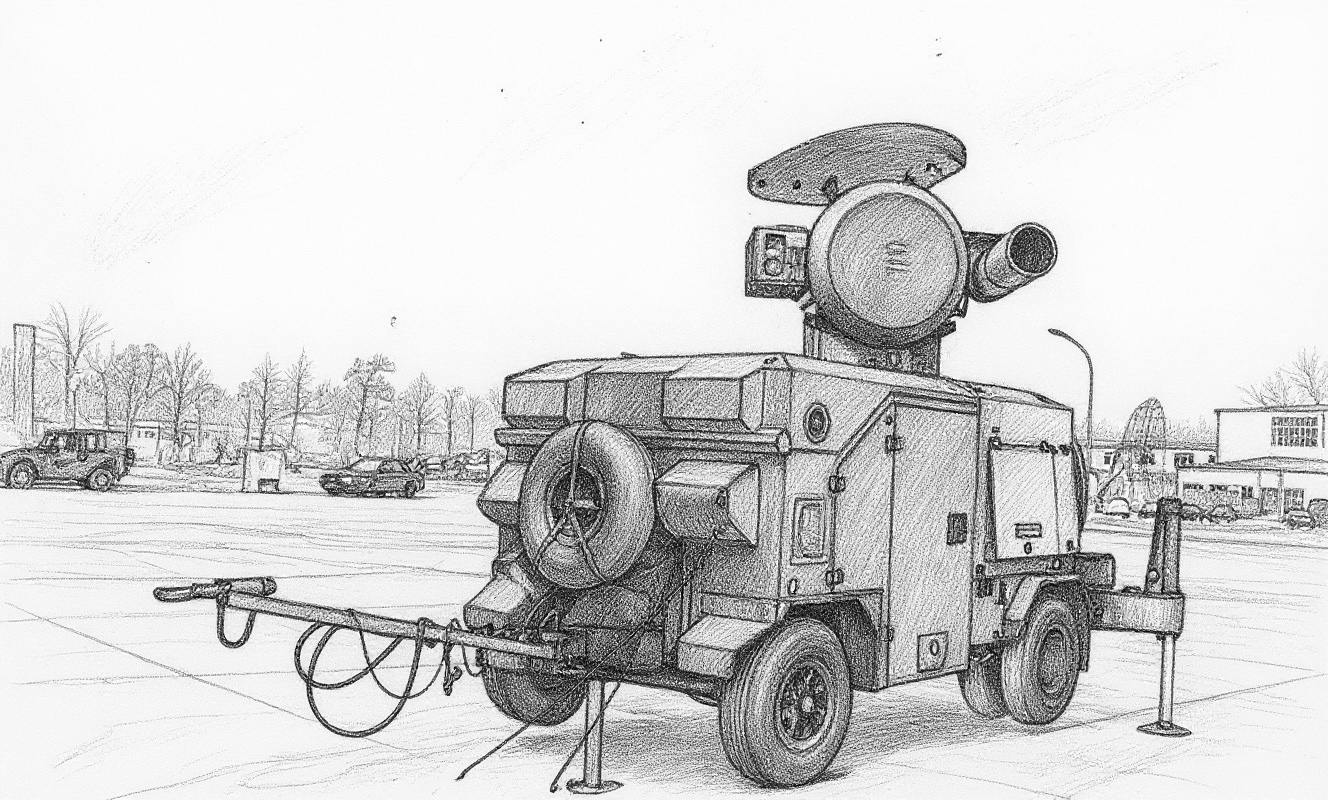
\includegraphics[width=\linewidth]{photos/skyguard.jpg}
%     % https://commons.wikimedia.org/wiki/File:Skyguard.jpg
% \end{figure}

The \hyperlink{table:fcr-units}{FCR Unit Table} summarizes the properties of FCR units.
As well as the basic properties common to all ground units, the table gives:
the FCR class;
the frequency band; and
the modifier to the hit roll.%
\note{FCR Units}{

    \noteparagraph{Bands}
    Radar frequencies are often referred to by the corresponding \href{https://en.wikipedia.org/wiki/Radio_spectrum\#EU,_NATO,_US_ECM_frequency_designations}{NATO} (post 1978) and \href{https://en.wikipedia.org/wiki/Radio_spectrum\#IEEE_radar_bands}{IEEE} band designations.
    \begin{center}
        \raisebox{-\depth}{
            \begin{tabular}{cc}
                \toprule
                Frequency&NATO\\
                (GHz)&Band\\
                \midrule
                \phantom{0}2--3\phantom{0}&E\\
                \phantom{0}3--4\phantom{0}&F\\
                \phantom{0}4--6\phantom{0}&G\\
                \phantom{0}6--8\phantom{0}&H\\
                \phantom{0}8--10\phantom{}&I\\
                \phantom{}10--20\phantom{}&J\\
                \phantom{}20--40\phantom{}&K\\
                \bottomrule
            \end{tabular}
        }
        \qquad
        \raisebox{-\depth}{
            \begin{tabular}{cc}
                \toprule
                Frequency&IEEE\\
                (GHz)&Band\\
                \midrule
                \phantom{0}1.55--3.9\phantom{00}&S\\
                \phantom{00}3.9--6.2\phantom{00}&C\\
                \phantom{00}6.2--10.9\phantom{0}&X\\
                \phantom{0}10.9--20.0\phantom{0}&Ku\\
                \phantom{0}20.0--36.0\phantom{0}&Ka\\
                \bottomrule
            \end{tabular}
        }
    \end{center}

    \noteparagraph{Frequencies}
    The table gives a summary of the frequencies of various FCRs along with the NATO and IEEE bands.
    Some radar systems use different individual radars for different roles.
    The roles are R for range, S for search, and T for tracking.
    The sources of the data are given in the entries for the individual radars.

    \begin{center}\scriptsize
        \begin{tabular}{lcccccccl}
            \toprule
            Radar&\vertical{Year}&\vertical{Role}&\vertical{Frequency (GHz)}&\vertical{NATO Band}&\vertical{IEEE Band}&\vertical{MTI}&\vertical{IFF}&Notes\\
            \midrule
            SCR-584&1944&S/T&2.7--2.8&E&S&N\\
            SCR-784&1945&S/T&2.7--2.8&E&S&N\\
            SON-4&1945&S/T&2.70-2.86&E&S&N\\
            Blue Cedar&1952&S/T&3.00--3.12&F&S&N&\\
            SON-9&1955&S/T&2.70--2.86&E&S&N\\
            SON-30&&S/T&---&E&S&N&Y\\
            SON-50&&S/T&9.25--9.70&I&X&N&Y\\
            Super Fledermaus&1965&S/T&8.6-9.6&I&X&Y&N&MTI from 1970\\
            Flycatcher&1979&S&9.2&I&X&Y&Y&MTI from 1992?\\
            &&T&9.2&I&X&---&---\\
            &&T&26.5--30&K&Ka&---&---&From 1992?\\
            Skyguard&1977&S/T&8.6--9.5&I&X&&Y\\
            \midrule
            M163/M167&1967&R&9.2--9.5&I&X&---&N\\
            Panhard M3 DCA&1975&S/R&---&E&S&Y&N\\
            ZSU 23-4&1965&S/T&14.6--15.6&J&Ku&N&Y&IFF from 1977\\
            Sinai 23&1992&S/R&---&E&S&Y&N\\
            Tunguska&1984&S&---&E&S&Y&Y\\
            &&T&---&J&X&---&---\\
            Gepard&1976&S&---&E&S&Y&Y\\
            &&T&---&J&Ku&---&---\\
            M51&1953&T&---&I&X&N\\
            \midrule
            AMX-13DCA&1969\\
            AMX-30SA&1979\\
            BOFI-R\\
            \bottomrule
        \end{tabular}
    \end{center}
}

\section{FCR-A}

\subsectionwithtwocounters{Towed and Mobile FCR-A Platoon}{towed FCR-A platoon}{mobile FCR-A platoon}

FCR-As typically use 1940s technology. They can be towed or mobile.

\subsectionwithcountercontinued{6}{SCR-584}

The SCR-584 is an early US towed FCR-A based on the British 3 GHz magnetron.
It replaced the much larger and less accurate SCR-268 and its basic technology was used in a series of successors.
The SCR-584 entered service with US and British anti-aircraft artillery units in 1944 and was commonly used to control batteries of 90~mm M2, QF 3.7~inch, 120~mm M1, and QF 5.5~inch guns.
It was also supplied to the Soviet Union and used to control batteries of 85~mm KS-12, and 100~mm KS-19 guns.%
\note{SCR-584}{
    I classify this as FCR-A as the SON-9 is derived from it.

    Wikipedia gives the frequency as 2.7--2.8 GHz (NATO E-band) and the search and tracking ranges for bomber-sized targets as 64~km and 29~km.

    Werrell mentions its use with the 90~mm and 3.7~inch guns against V-1s in 1944.

    \begin{notesources}
        \item Wikipedia on the \href{https://en.wikipedia.org/wiki/SCR-584_radar}{SCR-584}, \href{https://en.wikipedia.org/wiki/90_mm_gun_M1/M2/M3}{90~mm M1/M2 gun}, \href{https://en.wikipedia.org/wiki/120_mm_gun_M1}{120~mm M1 gun}, and \href{https://en.wikipedia.org/wiki/QF_3.7-inch_AA_gun}{QF 3.7~inch AA gun}.
        \item Werrell, K.P. (2005, Air University Press, 2nd edition): “\href{https://media.defense.gov/2017/Mar/31/2001725225/-1/-1/0/B_0028_WERRELL_ARCHIE_TO_SAM.PDF}{Archie to SAM}”.
        \item \href{https://www.radartutorial.eu/19.kartei/11.ancient4/karte001.en.html}{RadarTutorial}
        \item MobileRadar on the \href{https://www.mobileradar.org/radar_descptn_2.html}{SCR-784}
        \item
    \end{notesources}
}

\subsection{SCR-784}

The SCR-784 towed FCR-A is a more compact version of the SCR-584.
It entered service with the US Army in 1945, replacing the SCR-584 and controlling 90~mm M2 and 120~mm M1 guns.%
\note{SCR-784}{
    I classify this as FCR-A it is derived from the SCR-584.

    The earliest manuals I can find are from 1945, so I suspect that is its in-service date.

    \begin{notesources}
        \item Wikipedia on the \href{https://en.wikipedia.org/wiki/SCR-784_Radar}{SCR-784} and \href{https://en.wikipedia.org/wiki/SCR-584_radar}{SCR-584}.
        \item RadarTutorial on the \href{https://www.radartutorial.eu/19.kartei/11.ancient8/karte089.en.html}{SCR-784} and \href{https://www.radartutorial.eu/19.kartei/11.ancient4/karte001.en.html}{SCR-584}
        \item MobileRadar on the \href{https://www.mobileradar.org/radar_descptn_2.html}{SCR-584}
        \item RadioNerds on the \href{https://www.radionerds.com/index.php/SCR-784}{SCR-784}.
    \end{notesources}
}

\subsection{SON-4}

The Soviet SON-4 (Whiff) towed FCR-A is based on the SCR-584 radars supplied by the US during WW2.
It is commonly used with 85~mm KS-12 and 100~mm KS-19 batteries.
It entered services in the Soviet Army in 1948 and started to be replaced by the SON-9 in 1955.%
\note{SON-4}{
    I classify this as FCR-A it is derived from the SCR-584.

    RadioTutorial states that the frequency is 2.70--2.86 GHz.

    RadarTutorial states that it is a tracking radar, and was typically used with a P-8 (Knife Rest A) or P-10 (Knife Rest B) search radar.
    \begin{notesources}
        \item RadarTutorial on the \href{https://www.radartutorial.eu/19.kartei/11.ancient6/karte006.en.html}{SON-4}.
    \end{notesources}
}

\subsection{Blue Cedar}

The Blue Cedar or “Radar, Anti-Aircraft No.3 Mk.7” towed FCR-A is a post-war development of the Mk.4 radar with post-war technology, resulting in a more compact and reliable system.
It entered services with the British Army in 1952, controlling batteries of QF 3.7~inch and QF 5.25~inch guns, and served until these guns were retired in 1957. It also served with the Swiss Air Force from 1958, controlling 7.5~cm guns, until 1965, when the radars were replaced by Super Fledermaus systems and the guns by 35~mm Oerlikon GDFs. The radar was also used by the Netherlands, Sweden, Finland, and South Africa.%
\note{Blue Cedar}{

    I'm not sure whether this is a FCR-A or FCR-B.

    The frequency is 3.00--3.12 GHz (NATO F-band and IEEE S-band).

    The Swiss FCRs seem to have controlled 75~mm Flab Kan 38 L39 guns.

    \begin{notesources}
        \item Wikipedia on the \href{https://en.wikipedia.org/wiki/Radar,_Anti-Aircraft_No._3_Mk._7}{Blue Cedar}.
        \item RadarTutorial on the \href{https://www.radartutorial.eu/19.kartei/11.ancient7/karte019.en.html}{Blue Cedar}.
        \item Wikipedia on the \href{https://de.wikipedia.org/wiki/Fliegerabwehrtruppen}{Swiss Fliegerabwehrtruppen}.
    \end{notesources}
}

\subsection{SON-9}

The Soviet SON-9 (Fire Can) towed FCR-A was derived from the earlier SON-4, which in turn was derived from the US-supplied SCR-584.
It is commonly used with 57~mm S-60, 85~mm KS-12, 100~mm KS-19, and 130~mm KS-30 batteries.
The SON-9 entered service in 1955 with Soviet forces and was widely exported to Soviet allies.
It has seen combat, including with North Vietnam in the Vietnam War, Egypt and Syria in the 1967 War, the War of Attrition, and the 1973 War.%
\note{SON-9}{
    Wikipedia gives the frequency as 2.7--2.8 GHz (NATO E-band). RadarTutorial gives it as 2.7--2.86 GHz.

    Wikipedia states this was used with the 57, 85, 100, and 130~mm guns and was widely deployed in the Vietnam War. In {\TSOH} the 57~mm S-60 and 85~mm KS-12 are often combined with an FCR-A, presumably the SON-9.

    \begin{notesources}
        \item Wikipedia on the \href{https://en.wikipedia.org/wiki/SON-9}{SON-9}.
        \item \href{https://www.radartutorial.eu/19.kartei/11.ancient6/karte007.en.html}{RadarTutorial}
    \end{notesources}
}

\subsection{SON-30}

The Soviet SON-30 (Fire Wheel) towed FCR-B was derived from the earlier SON-9.
It entered service in 1957 and was used to control batteries of 130~mm KS-30 guns.%
\note{SON-30}{

    This looks very similar to the SON-9.

    RadarTutorial gives the frequency as S band.

    The photo on RadioTutorial shows an integrated IFF system.

    Wikipedia and RadarTutorial both state it was used for 130 mm guns, but do not mention others.

    RadarTutorial states that it had replaced the SON-4 and SON-9 by 1957, but the SON-9 only entered service in 1955. I suspect that it entered service in 1957.

    Foss (p.~185) states that it was used for 130 mm guns.

    \begin{notesources}
        \item Wikipedia on the \href{https://en.wikipedia.org/wiki/SON-30}{SON-30}.
        \item RadarTutorial on the \href{https://www.radartutorial.eu/19.kartei/11.ancient6/karte009.en.html}{SON-30}.
        \item Foss, Christopher F., 1974 (London : Allan): “\href{https://archive.org/details/artilleryofworld0000foss_u1u7/page/184/mode/2up?q=\%22SON-9\%22}{Artillery of the World}”.
    \end{notesources}
}

\pagebreak
\section{FCR-B}

\subsectionwithtwocounters{Towed and Mobile FCR-B Platoon}{towed FCR-B platoon}{mobile FCR-B platoon}

FCR-Bs typically use 1950s technology.
They can be towed or mobile.

\subsectionwithcountercontinued{6}{SON-50}

The SON-50 (Flap Wheel) mobile FCR-B is new development and a contemporary of the RPK-2/1RL33 (Gun Dish) radar used in the ZSU-23-4.
It has an integrated IFF system.
It is used to control batteries of S-60 57~mm and KS-30 130~mm guns.
It entered service in the 1960s.%
\note{SON-50}{

    This is truck-mounted.

    RadarTutorial gives the frequency as 9.25--9.7 GHz (X band).

    The photo on RadioTutorial shows an integrated IFF system.

    RadarTutorial states it was used for 57 and 130 mm guns. Wikipedia states it was used for 57 mm guns.

    RadarTutorial states that it is mounted on a URAL-375. Wikipedia then states that this was produced from 1961 to 1993. The in-service data can be no earlier than 1961. I guess it entered service in the 1960s; by the 1970s I think the focus had moved to SAMs.

    Chant (p.\ 253) states that the SON-50 is believed to be derived from the Gun Dish radar on the ZSU-23-4 and has a TV back-up. I note, however, that the frequencies are very different: Flap Wheel is E band and Gun Dish is J band.

    \begin{notesources}
        \item Wikipedia on the \href{https://en.wikipedia.org/wiki/SON-50}{SON-50} and \href{https://en.wikipedia.org/wiki/Ural-375}{Ural-375}
        \item RadarTutorial on the \href{https://www.radartutorial.eu/19.kartei/11.ancient4/karte087.en.html}{SON-50}.
        \item Chant, Christopher, 1989 (Brassey's Defence Publishers): “\href{https://books.google.com.mx/books?id=C3osAAAAYAAJ&q=\%22Fire+Wheel\%22+\%22SON-30\%22&redir_esc=y}{Air Defence Systems and Weapons World AAA and SAM Systems in the 1990s}”.
    \end{notesources}
}

\section{FCR-C}

\subsectionwithtwocounters{Towed and Mobile FCR-C Platoon}{towed FCR-C platoon}{mobile FCR-C platoon}

FCR-Cs typically use 1960s technology.
They can be towed or mobile.

\subsectionwithcountercontinued{6}{Super Fledermaus}

The Contraves Super Fledermaus FCR-C can control a section of two Oerlikon GDF 35~mm guns; it cannot control a whole battery.
It entered service in 1965 with the Swiss Air Force and also was used by the Argentine Air Force, Brazil, Iran, Israel, Japan, and South Africa.
It was used by Israel in the 1967 Six Day War and afterward with the Bofors 40~mm L/70 gun to defend strategic sites.
It also saw combat with the Argentine Air Force in the 1982 South Atlantic War controlling Oerlikon GDF guns in the defense of BAM Malvinas (Port Stanley Airport).%
\note{Super Fledermaus}{
    Wikipedia states there were two versions: the Feuerleitgerät (FLt Gt) 63 (from 1965) and the Feuerleitgerät 69 (from 1970). The latter had “background clutter suppression,” which probably is equivalent to MTI.

    Wikipedia states that it can control \emph{two} Oerlikon GDF mounts, hence the restriction to controlling sections and not batteries.

    Wikipedia also states these the prototype of the Gepard used a Flt Gt 63. Since the FCR-W radar of the Gepard is equivalent to a \plus{2} modifier and has VF frequency, it corresponds to an FCR-C. We assume the Super Fledermaus does too.

    The Wikipedia page on the Super Fledermaus gives the frequency as 8.6--9.6~GHz (old NATO X-band), but also states that its search function operates in the E/F bands (2--4 GHz) and tracking function in the J band (10--20 GHz).

    The service history is from Wikipedia and Singh (for Israeli use).

    \begin{notesources}
        \item Wikipedia on the \href{https://en.wikipedia.org/wiki/Super_Fledermaus}{Super Fledermaus} and \href{https://en.wikipedia.org/wiki/Oerlikon_GDF\#Super_Fledermaus}{its use with the Oerlikon GDF}.
        \item Singh, M. (Pen \& Sword, 2020): “Anti-Aircraft Artillery in Combat 1950--1972: Air Defence in the Jet Age”.
    \end{notesources}
}

\subsection{Flycatcher}

The Signaal Flycatcher FCR-C can control up to six Bofors L/60 or L/70 guns or SAM launchers.
Flycatcher entered service with the Royal Netherlands Air Force in 1979, serving for airfield defense and each controlling three modified Bofors 40~mm L/70 gun mounts. It subsequently served with the Indian Armed Forces from 1985, the Irish Defense Forces from 2003, the Royal Netherlands Army from 1987, the Thai Armed Forces from 1981, Turkey, and Venezuela.%
\note{Flycatcher}{
    Flycatcher is similar to the Cheetah radar, so presumably FCR-C.

    According to Wikipedia, the search radar is NATO I/J band and the tracking radar is NATO K band. RadioTutorial states the search frequency is 9.2 GHz (NATO I band) and the tracking frequency is either I or K band.
    Van Elk states the tracking radar is an independent pulse-Doppler 26.5--31 GHz (old-NATO Ka band) system, but this seems to be referring to an upgrade in 1992. He also mentions that the radar is used in the Goalkeeper CIWS, and the Wikipedia page on this states it searches in I band and tracks in both I and K bands.
    I conclude:
    \begin{itemize}
        \item Search is 9.2 GHz (I band)
        \item Tracking is 9.2 GHz (I band) or 26.5--31 GHz (K band)
    \end{itemize}

    Van Elk states that it has IFF and directed a maximum of 3 cannons or missile launchers.

    Van Elk states that it succeeded the HSA L4/5 radar.

    \begin{notesources}
        \item Wikipedia on the \href{https://en.wikipedia.org/wiki/Flycatcher_(radar)}{Flycatcher}.
        \item van Elk, Bert (2020): \href{https://magazines.defensie.nl/materieelgezien/2020/09/06_flycatche}{Terug naar de toekomst: De Flycatcher}.
        \item \href{https://www.radartutorial.eu/19.kartei/06.missile/karte012.en.html}{RadarTutorial}
    \end{notesources}
}

\section{FCR-D}

\subsectionwithtwocounters{Towed and Mobile FCR-D Platoon}{towed FCR-D platoon}{mobile FCR-D platoon}

FCR-Ds typically use 1970s technology. They can be towed or mobile.

\subsectionwithcountercontinued{6}{Skyguard}

The Contraves Skyguard FCR-D can control two Oerlikon GDF 35~mm guns and additionally a SAM launcher with AIM-9 Sparrow, RIM-9 Sea Sparrow, or Aspide missiles.
Skyguard entered service in 1977 with the Swiss Air Force.
It was subsequently very widely exported and used by the Argentine Army, Austria, Bahrain, Bangladesh, Brazil, Canada, Chile, China, Cyprus, Egypt, Greece, Indonesia, Iran, Italy, South Korea, Kuwait, Malaysia, Oman, Pakistan, Saudi Arabia, Spain, Taiwan, and the UK.
It saw combat with the Argentine Army in the 1982 South Atlantic War in the defense of BAM Malvinas (Port Stanley Airport) and BAM Condor (Goose Green Airfield) controlling Oerlikon GDF 35~mm guns.%
\note{Skyguard}{

    RadarTutorial states that the frequency is 8.6--9.5 GHz (NATO I-band or IEEE X-band). The description of the system suggests that both search and tracking radars use the same frequency.

    \begin{notesources}
        \item Wikipedia on the \href{https://en.wikipedia.org/wiki/Oerlikon_GDF\#Skyguard}{Skyguard's use with the Oerlikon GDF}.
        \item \href{https://www.radartutorial.eu/19.kartei/11.ancient6/karte059.en.html}{RadarTutorial}
    \end{notesources}
}

\begin{table}
    \caption*{\hypertarget{table:fcr-units}{FCR Unit Table}}
    \centering
    \footnotesize
    \input{table-fcr-units.tex}
    \label{table:fcr-units}
\end{table}
